\subsection{Generate Language Implementation}

Now that the initial grammar of the language has been defined it is time to test
the language. Xtext ships with a code generator which generates all the glue
code needed for the language implementation.

To generate the code, we need to execute the generator workflow
\texttt{GenerateQlDsl.mwe2}. For this, select the workflow file, open the context menu
and select \emph{Run As / MWE2 Workflow}.

The generator will print some information to the Console, and finally it should
print \texttt{``Done.''}.

\begin{lstlisting}
0    [main] INFO  lipse.emf.mwe.utils.StandaloneSetup  - Registering platform
uri ....
   ...
13727 [main] INFO  .emf.mwe2.runtime.workflow.Workflow  - Done.
\end{lstlisting}

After successful execution the projects will be filled with implementation code.
Code that will be regenerated each time the generator is executed will go to the
source folder \texttt{/src-gen} (in all three projects), whereas code generated to
\texttt{/src} will be generated only once as skeleton. It is safe to edit these
classes.

Xtext follows the Generation Gap
Pattern\footnote{\url{http://heikobehrens.net/2009/04/23/generation-gap-pattern/}}:
Generated code is based on the Xtext API. Manual code is separated from
generated code. Often manual classes are derived from generated classes to allow
overriding of generated code or adding functionality.

Investigate the generated code a bit. Some pieces to mention:
\paragraph{Runtime Project - folder \texttt{src}}
\begin{itemize}
\item The class \texttt{QlDslRuntimeModule} is a Guice configuration.
Guice\footnote{\url{http://code.google.com/p/google-guice/}} is a famous
Dependency Injection\footnote{\url{http://en.wikipedia.org/wiki/Dependency_injection}} framework in Java. 
Xtext makes heavy use of Dependency Injection, which in turn allows to exchange
nearly every bit of the framework for customizing or to work around limitations,
if necessary, without the need to change the framework itself.
\item Class \texttt{QlDslStandaloneSetup} is needed when using the language in
``standalone mode'', i.e. without an Eclipse environment. Eclipse plugins, like
Xtext and the language plugin, usually need an OSGi container as execution
environment. Xtext is designed to be executable without the need to be
deployed into an OSGi container, but for this certain registrations are
required which an OSGi container would usually provide automatically. This is
especially useful when Xtext based languages are used in build environments or
other IDEs.
\item Class \texttt{QlDslFormatter} allows the implementation of a declarative
code formatter for the DSL.
\item File \texttt{QlDslJvmModelInferrer.xtend} is a class implemented with the
Xtend language. The JVM Model Inferrer will play an important role later when we
introduce expressions and code generation.
\item Class QlDslJavaValidation allows the implementation of validation rules
for the DSL.
\end{itemize}


\paragraph{Runtime Project - folder \texttt{src-gen}}
\begin{itemize}
  \item The Ecore metamodel is generated to file \texttt{QlDsl.ecore}.

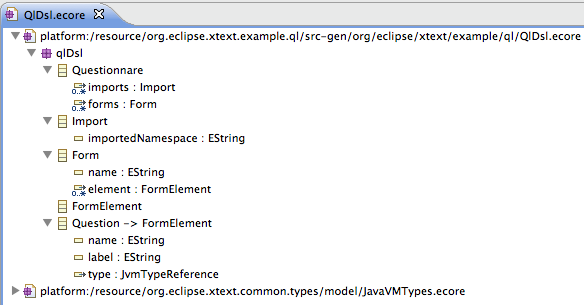
\includegraphics[width=16cm]{./images/chapter01/QlDsl_ecore.png}

  \item The Java implementation code for the metamodel can be found in the
  package \texttt{org.eclipse.xtext.example.ql.qlDsl}.
  \item The package \texttt{org.eclipse.xtext.example.ql.parser.antlr.internal}
  contains an ANTLR3\footnote{\url{http://www.antlr.org}} grammar and the Lexer
  and Parser classes generated from it.
\end{itemize}

